\section{Simulations}
\label{sec:simulation}

The simulator models the interarrival time between packets to transmit to a station with an exponential distribution.
The size of each packet is extracted from a uniform distribution between $32$ and $1460 B$.
Each station has a limited amount of memory, so it can store at most $2$ packets in a queue.
Packets that do not fit in the queue are discarded.
All simulations use the same network topology, shown in \cref{fig:network}.
Each simulation is run with multiple seeds for the pseudonumber generator in order to get more robust results.

\begin{figure}[ht]
	\centering
	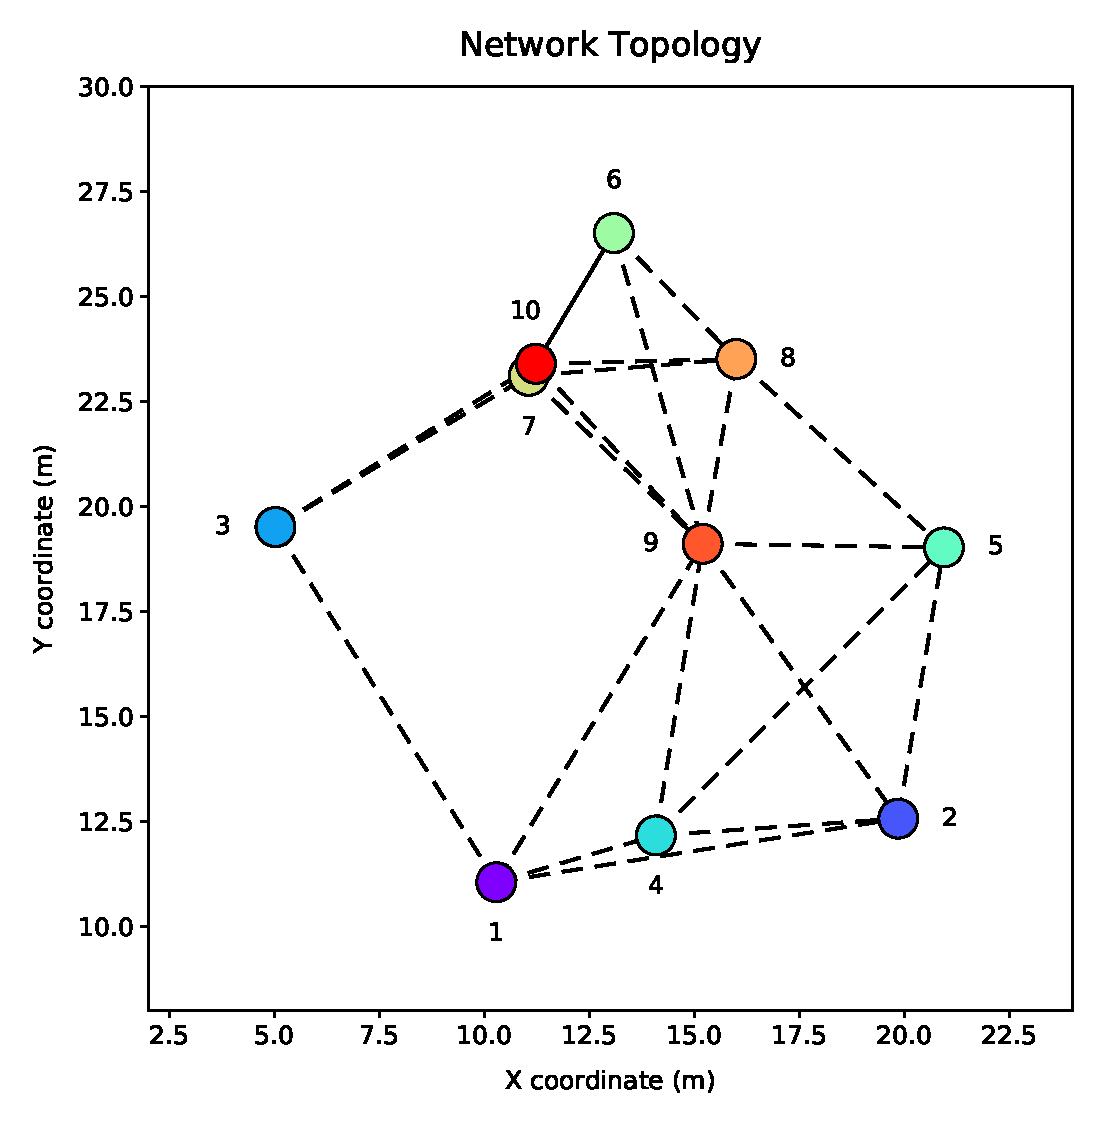
\includegraphics[width=0.9\columnwidth]{figures/plots/topology}
	\caption{The plot show the topology of the network used to run all simulations. Only nodes connected by a dashed line can communicated with each other.}
	\label{fig:network}
\end{figure}
